\documentclass{beamer}

\usepackage[utf8]{inputenc}
\usepackage[T1]{fontenc}
\usepackage{adjustbox}
\usepackage{booktabs}
\usepackage{graphicx}
\usepackage{listings}
\usepackage{lstlinebgrd}
\usepackage{multirow}
\usepackage{subcaption}
\usepackage{tikz}
\usepackage{ulem}

\fontseries{bx}
\selectfont

\setlength{\tabcolsep}{18pt}

\graphicspath{{./gfx/}}

\usetikzlibrary{fit}

\usetheme{Madrid}

\title[Cloud MCS]{Improving Cloud Simulation Using the Monte-Carlo Method}
\author[Luke Bertot]{\underline{Luke Bertot} \and Stéphane Genaud \and Julien Gossa\\}
\institute[ICPS]{%
	\{lbertot,genaud,gossa\}@unistra.fr\\
	\medskip{}
	ICPS -- Scientific and Parallel Computing research group\\ 
	at ICube, University of Strasbourg CNRS}

\date[Euro-Par 2018]{Euro-Par, August 2018}

\titlegraphic{\raisebox{-0.5\height}{
\includegraphics[width=1.5cm]{/icube-png.png}}\hspace*{1cm}~\raisebox{-0.5\height}{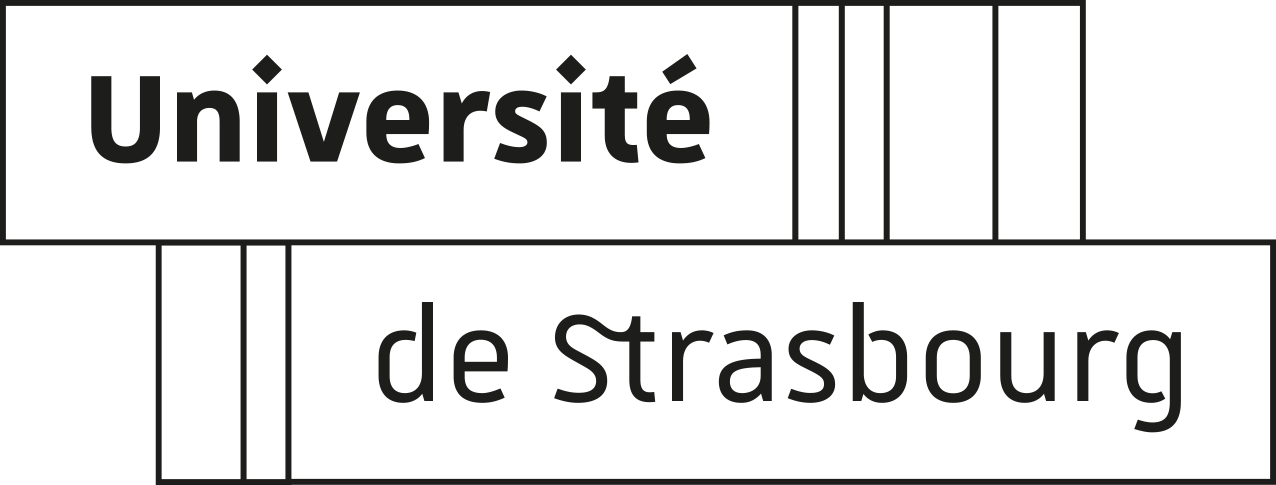
\includegraphics[width=2cm]{uds.png}}\hspace*{1cm}~\raisebox{-0.5\height}{
\includegraphics[width=1.5cm]{Logo_CNRS.png}}}

\setbeamertemplate{navigation symbols}{}%remove navigation symbols

\newcommand\blfootnote[1]{%
  \begingroup
  \renewcommand\thefootnote{}\footnote{#1}%
  \addtocounter{footnote}{-1}%
  \endgroup
}


\AtBeginSection[]{%
	\begin{frame}
		\begin{beamercolorbox}[sep=8pt,center,shadow=true,rounded=true]{title}
			\usebeamerfont{title}\insertsectionhead\par
		\end{beamercolorbox}
	 \end{frame}
}

\begin{document}

\begin{frame}
\maketitle{}
\end{frame}

\begin{frame}
	\frametitle{Outline}
	\tableofcontents
\end{frame}

\section{Cloud Brokering}

\begin{frame}
	preesent workflows we are working with.
\end{frame}

\begin{frame}
	( present schlouder ) 
\end{frame}

\begin{frame}
	present schdeules, and difficulties around scheduling
\end{frame}

%\section{Cloud Simulations}

\begin{frame}
	present simschlouder limits to that approach
\end{frame}

\begin{frame}
	?? numerical stochastic simulations. 	
\end{frame}

\section{Monte-Carlo Simulations}

\begin{frame}
	MC process
\end{frame}

\begin{frame}
	Experimental rational	(+modele simple)
\end{frame}

\begin{frame}
	our experimental setup (in vivo/in silico)
\end{frame}

\begin{frame}
	real runs
\end{frame}

\begin{frame}
 	input model +(Leitner)
\end{frame}

\section{Results}

\begin{frame}
	fig3 + table 1
\end{frame}

\begin{frame}
	fig4 
\end{frame}

\begin{frame}
	number iter
\end{frame}
\section{conclusion}
\end{document}
% vim: spell spelllang=en
